\documentclass[10pt,twocolumn,letterpaper]{article}

\usepackage{cvpr}
\usepackage{times}
\usepackage{epsfig}
\usepackage{graphicx}
\usepackage{amsmath}
\usepackage{amssymb}

% Include other packages here, before hyperref.

% If you comment hyperref and then uncomment it, you should delete
% egpaper.aux before re-running latex.  (Or just hit 'q' on the first latex
% run, let it finish, and you should be clear).
\usepackage[breaklinks=true,bookmarks=false]{hyperref}

\cvprfinalcopy % *** Uncomment this line for the final submission

\def\cvprPaperID{****} % *** Enter the CVPR Paper ID here
\def\httilde{\mbox{\tt\raisebox{-.5ex}{\symbol{126}}}}

% Pages are numbered in submission mode, and unnumbered in camera-ready
%\ifcvprfinal\pagestyle{empty}\fi
\setcounter{page}{1}
\begin{document}

%%%%%%%%% TITLE
\title{AFEW Competition of Emotion Recognition}

\author{Cao Kaidi\\
EE43\\
2014012282
\and
Lin Ji\\
EE43\\
2014011097
\and
Yan Jingkai\\
EE46\\
2014011192
}

\maketitle
%\thispagestyle{empty}

%%%%%%%%% ABSTRACT
\begin{abstract}
   TO BE DONE
\end{abstract}

%%%%%%%%% BODY TEXT
\section{Introduction}

\begin{figure*}[htpb]
	\centering
	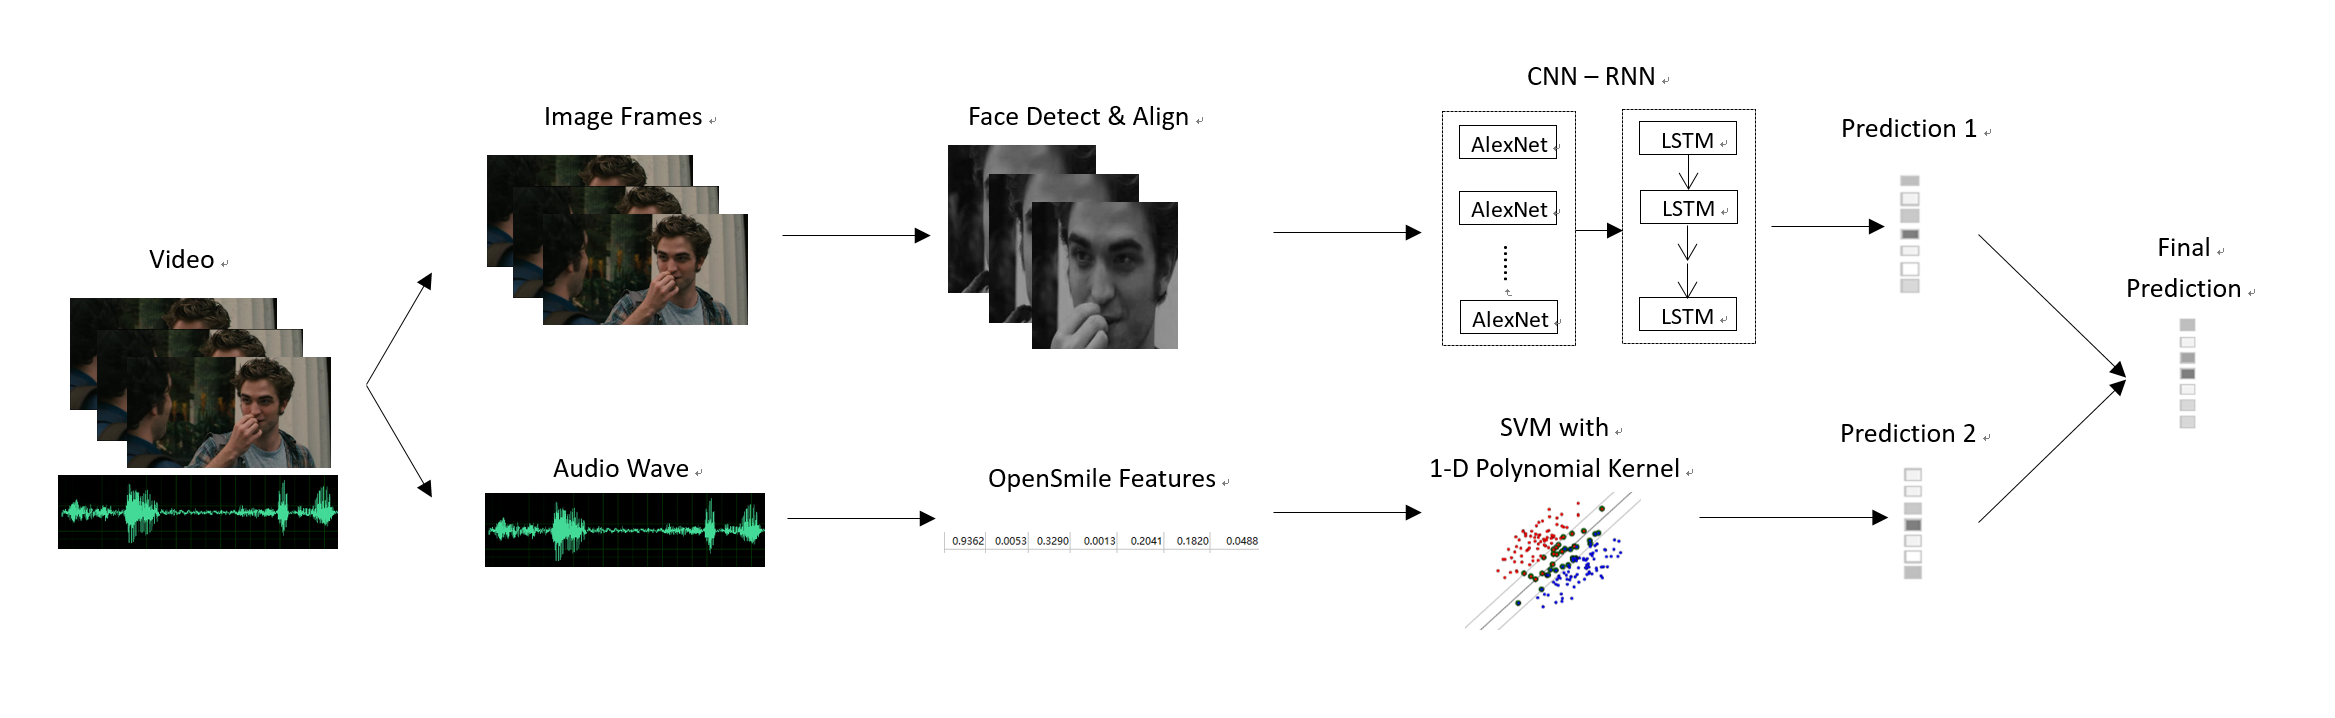
\includegraphics[width = \textwidth]{pic/pipeline.png}
	\caption{Pipeline}
\end{figure*}

\section{Preprocessing}

As for visual part, it could be easily observed that there exists a large amount of unrelated information such as background, illumination, color, etc. that we humans do not need to reference while deciding a person's emotion. Thus, it would be reasonable that we conduct preprocessing procedure before feeding frames into neural network. Here we perform face detection and face alignment, which is a common process in tasks like face verification.

In face detection part, we tested two open source software. Openface \cite{amos2016openface} is a Python and Torch implementation of face recognition with deep neural networks and is based on the CVPR 2015 paper FaceNet \cite{schroff2015facenet}. A sad news is that its detection toolkit is currently developed on dlib \cite{king2009dlib}, which couldn't support CUDA, resulting in a huge time cost. One remedy we attempted on this software is to use thread pool parallel computing. By applying 8 threads concurrently we are able to compress the detection time of a video clip into 2 seconds or so. However, this software has another big issue that is basically not tolerable, detection recall.

Thus we found a more state of the art implementation of face detection, named Joint Face Detection and Alignment using Multi-task Cascaded Convolutional Neural Networks \cite{7553523}. It's a matcaffe implementation, which fits our environment quite well. More importantly, its detection recall is far more satisfying, so that we use this tool in our final submission. We provide our detection recall test result in Table 1. Not detected means not a single face was detected among all frames. 

\begin{table}[htpb]
	\begin{center}
		\begin{tabular}{|l|c|c|}
			\hline
			Method & Not Detected & Total Frames\\
			\hline\hline
			OpenFace & 75 & 383\\
			\hline
			MTCNN & 4 & 383\\
			\hline
		\end{tabular}
	\end{center}
	\caption{Detection Results Tested on Val Set}
\end{table}

Since MTCNN was originally designed to generate detection and alignment result simultaneously, it is quite intuitive to apply affine transformation given 5 facial landmarks.

\section{Learn Audio Signals}

Audio signal is another important component in video recognition. In the case of AFEW, we discover that the audio segments from movie clips vary significantly from each other, including the existence of speech and background music. Therefore, we predict the audio recognition result to be less accurate than the video dimension. Nonetheless, a proper exploitation of audio features can also provide reference to our recognition and improve the performance.

We adopt the Opensmile toolbox \cite{eyben2010opensmile} for audio feature extraction. The feature configuration applied here is \texttt{emobase2010}, which projects each wave file onto a 1583-dimension vector, with features including loudness, MFCC values, etc. Insipired by the work of \cite{fan2016video} Then we apply an SVM classifier to learn audio features from the training data.

In the selection of SVM parameters, we experimented with several types of kernel functions including linear, polynomial and RBF, and discovered that linear kernel yields the best performance. The choice of optimal parameters such as cost and weight are found using grid search method.

% To be added, transfrom decision value to probability distribution

\section{Model Fusion}

Referencing previous studies, prediction accuracy given by audio models are usually worse than video models, but it could be taken as decent feature supplement to video model, which usually results in an increase in model performance.

Here's what we do, we performance softmax manipulation on both video and audio outputs and get two probability distributions. We model our final probability prediction by function

\begin{equation}
Prob_{final} = Prob_{video} + t \times Prob_{video} 
\end{equation}

We selected the value of $t$ by investigating the performance of $t$ from $0$ to $1$ with a step of $0.01$ and got the curve shown in . From the figure we decided to choose the t value as $t=0.25$. The argmax of $Prob_{final}$ will serve as our final prediction.

\begin{figure}[t]
	\centering
	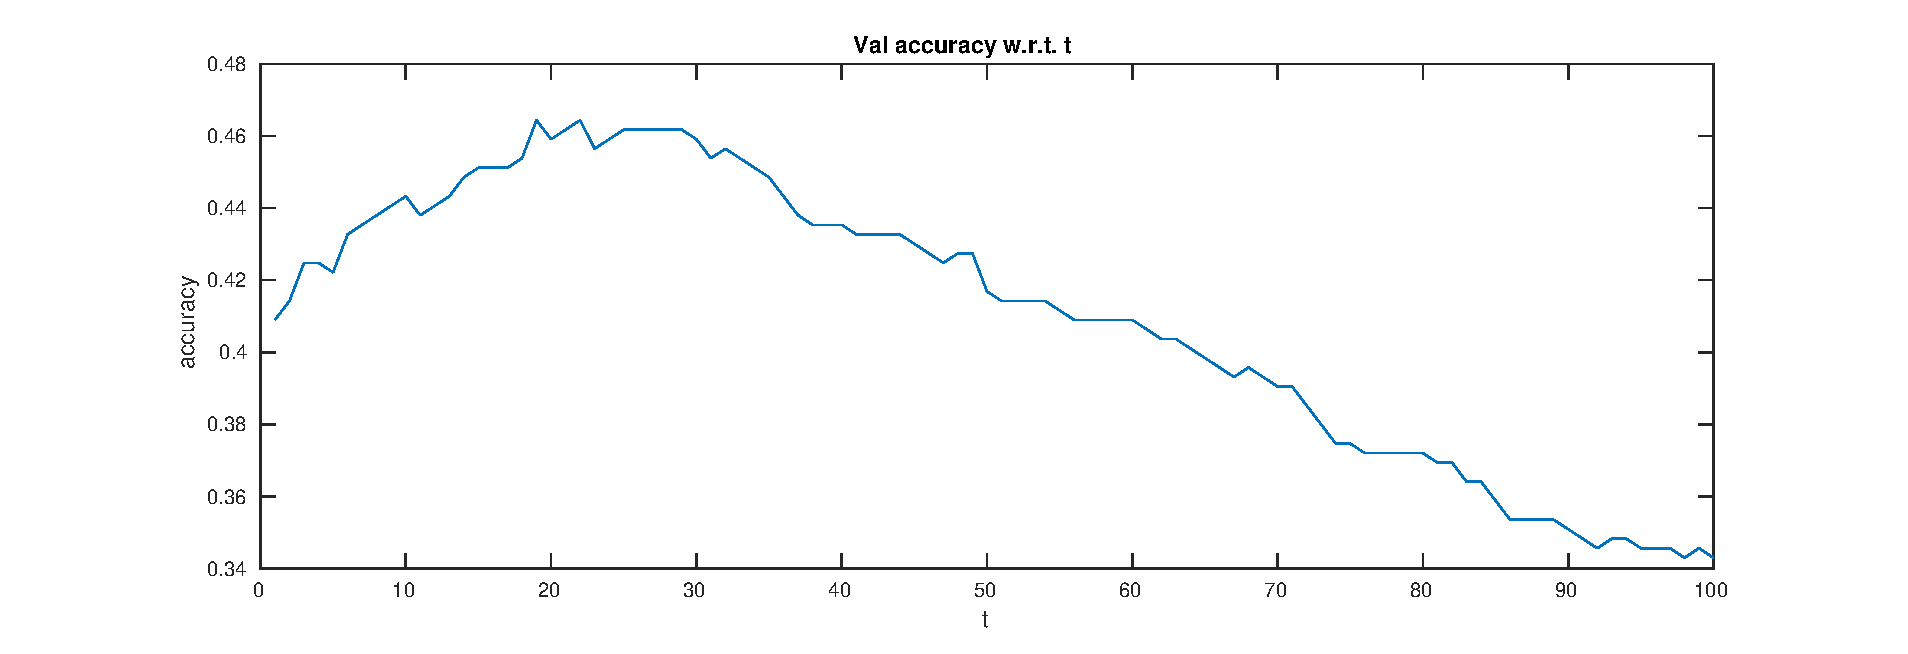
\includegraphics[width = 8cm]{pic/t_selection.eps}
	\caption{t selection curve}
\end{figure}

Another implementation worth clarifying is that our audio model will always have a prediction while the video model will fail to do so if there's not a single face detected by MTCNN. In this case, we'll produce results solely by audio model, which is still higher than random guess. And from Table 1. we can see that this detection model rarely fails. 

\section{Experiment}

\section{Conclusion}

\section{Acknowledgement}

Image-based caffe models are all trained by Lin Ji, Yan Jingkai has accomplished audio model, Cao Kaidi is responsible for video preprocessing, model fusion and deployment.

{\small
\bibliographystyle{ieee}
\bibliography{AFEW}
}

\end{document}
